% Created 2018-05-08 Ter 15:57
\documentclass[a4paper, 12pt]{report}
\usepackage[utf8]{inputenc}
\usepackage[T1]{fontenc}
\usepackage{fixltx2e}
\usepackage{graphicx}
\usepackage{longtable}
\usepackage{float}
\usepackage{wrapfig}
\usepackage{rotating}
\usepackage[normalem]{ulem}
\usepackage{amsmath}
\usepackage{textcomp}
\usepackage{marvosym}
\usepackage{wasysym}
\usepackage{amssymb}
\usepackage{hyperref}
\tolerance=1000
\usepackage{minted}
\usepackage{indentfirst}
\usepackage[portuguese, ]{babel}
\usepackage{setspace}
\usepackage{fancyhdr}
\usepackage{float}
\usepackage{url}
\usepackage[utf8]{inputenc}
\usepackage{minted}
\renewcommand\listingscaption{Código}
\author{Rafael Campos Nunes}
\date{8 de abril de 2018}
\title{Análise sobre Algoritmos de Ordenação Interna}
\hypersetup{
  pdfkeywords={},
  pdfsubject={},
  pdfcreator={Emacs 25.3.1 (Org mode 8.2.10)}}
\begin{document}

\maketitle
\begin{figure}
  \centering
  
\includegraphics[width=4in]{./img/utfpr_black.png}
\end{figure}

\begin{abstract}
Este trabalho tem como intento apresentar o significado de algoritmo utilizado
em dispositivos computacionais e colocar em destaque o estudo de algoritmos de
ordenação interna. Esse estudo será feito utilizando dois parâmetros: sendo o
primeiro  tamanho da entrada e o segundo o quão desordenada está dessa entrada.
Por fim, este estudo apresenta uma análise global sobre os algoritmos de
ordenação evidenciando os melhores e os piores algoritmos em cada ponto de
análise.
\end{abstract}

\onehalfspacing

\setcounter{tocdepth}{2}
\tableofcontents

\part{Introdução}
\label{sec-1}
Atualmente se emprega a utilização da palavra \emph{algoritmos} para denotar um
conjunto de passos para se realizar uma tarefa. Embora tal definição esteja
correta, essa definição não é suficientemente rígida para os campos de estudo
exatos.

Um desses campos, a ciência da computação, utiliza-se do conceito de algoritmo
para definir instruções computacionais, isto é, instruções realizadas em um
dispositivo capaz de realizar cálculos tal qual é feito à mão. Pela natureza
dos computadores, esses algoritmos não podem ser descritos da mesma maneira
como são descritas receitas de bolo, a exemplo.

Os algoritmos computacionais são, portanto, nada mais que um conjunto de
instruções para um fim, de forma que tais instruções são descritas a um nível
de precisão necessário para um computar executá-las. A partir dessa definição
pode-se observar outro aspecto de algoritmos: a recorrência com que estão
presentes no século XXI.

É notória a utilização em grande escala de computadores, tablets e smartphones
pelo sociedade atual, contudo, os algoritmos que realizam as diversas tarefas
desses dispositivos são invisíveis aos olhos do utilizador. Tais algoritmos são
objeto de estudo nesse relatório, mais especificamente, os que tangem a
ordenção de dados.

Os algoritmos de ordenação tem como finalidade a ordenação de dados, isto é,
dada uma entrada de dados, chamada doravante de \emph{instância}, ele reorganiza os
dados de maneira que obedeçam uma característica definida \emph{a priori} e retorna
uma instância com os respectivos dados ordenados.

\part{Referencial teórico}
\label{sec-2}
Informalmente um algoritmo é qualquer procedimento computacional bem definido
que tomando como entrada um conjunto de dados A transforma tal conjunto em
um conjunto de dados B, sendo este considerado o resultado ou saída de um
algoritmo. Também pode-se considerar um algoritmo como uma ferramenta para
resolver um problema computacional bem especificado\footnote{CORMEN et al. Algoritmos p.3}.

Além de um algoritmo ser uma ferramenta com propósito excertado no parágrafo
anterior, ele também pode ser definido como tecnologia. Isso pode ser explicado
colocando os diversos tipos de algoritmos diferentes para resolver uma mesma
tarefa, a partir disso pode se observar a diferença de performance, tanto de
tempo de execução e utilização de recursos como a memória do dispositivo
computacional. Um algoritmo eficiente utilizará esses recursos, que são
finitos, eficientemente, ou seja, fazendo o melhor aproveitamento tanto da
unidade de processamento central como da memória primária ou de armazenamento
em massa\footnote{CORMEN et al. Algoritmos p.7-9}.

Considerando os problemas de ordenação de dados têm-se os algoritmos de
ordenação cujo propósito é reorganizar os elementos de uma instância sob uma
restrição definida pelo programador. Esses, por sua vez, podem ser
categorizados em dois grupos: os algoritmos de ordenação interna e os
algoritmos de ordenação externa. O primeiro tange os algoritmos que se utilizam
exclusivamente da memória primária do computador a memória de acesso randômico
(RAM) e serão objetos de análise neste relatório. A segunda categoria abarca os
algoritmos que utilizam, além da memória primária, a memória de armazenamento
em massa. Este fato decorre da limitação física de armazenar todos os dados a
serem ordenados na RAM.

Tomando os dois grupos de algoritmos de ordenação tem-se, ainda, outras
características que são inerentes a esses como a estabilidade ou não
estabilidade do algoritmo e o método utilizado para a ordenação. A propriedade
de estabilidade de um algoritmo confere a este a não troca de posição de chaves
cujos valores são iguais, ou seja, a posição relativa dessas chaves é mantida.
O método de ordenação descreve como o algoritmo rearranja os elementos, seja
por partição, mesclagem, seleção ou troca.

Por fim, ao lado dos dois grupos expostos anteriormente, é válido ressaltar
algumas estratégias que são extensivamente utilizadas para resolver, da melhor
maneira, problemas de ordenação, mas não limitado a eles. Elas compreendem a
forma de como os algoritmos resolvem o problema, e são: estratégia gulosa,
programação dinâmica e divisão e conquista. Segundo Toscani e Veloso, a
primeira estratégia é útil para resolução de problemas de otimização
combinatória cujas soluções podem ser alcançadas por meio de sequências de
decisões. A segunda é aplicada a problemas que não é fácil se chegar a uma
sequência ótima de decisões sem testar as várias sequências possíveis e a
terceira estratégia é a decomposição de um problema em várias partes para então
resolver as várias partes e, por fim, recombinar as partes obtendo a solução
do problema\footnote{TOSCANI, VELOSO. Complexidade de Algoritmos p.188-190}.

\chapter{Algoritmos quadráticos}
\label{sec-2-1}
Algoritmos quadráticos são, a rigor, algoritmos onde a grandeza assintótica tem
crescimento proporcional a $n^2$, dessa forma pode-se observar o melhor, médio
e pior caso desses algoritmos com pelo menos um deles contendo essa grandeza.

É importante salientar que, embora a grandeza assintótica desses algoritmos
sejam iguais, eles não necessariamente tem a mesma performance quando
colocados em execução sobre a mesma quantidade de dados, ou seja, sobre uma
instância de mesmo tamanho. Isto é consequência do fato de que a notação
assintótica despreza termos absolutos em seu cálculo.

Portanto, para saber exatamente qual de dois algoritmos com mesma ordem de
grandeza assintótica é melhor, é necessário realizar o cálculo em termos
absolutos com relação a trocas ou deslocamentos de elementos feitos por estes.

\section{Bubble Sort}
\label{sec-2-1-1}
O Bubblesort é um algoritmo de ordenação estável e comparativo que realiza a
trocas de chaves adjacentes à posição de ordenação de acordo com o valor
dessas.

Esse algoritmo é considerado o mais lento em termos de execução pois sua
execução é afetada por dois motivos: a quantidade excessiva de comparações e
de trocas necessárias. Tais motivos conferem o título de algorimo de ordenação
mais lento dentre os destacados nesse trabalho.

A seguir, pode-se visualizar o código em C++ de sua implementação. O algoritmo
itera sobre a instância de tamanho $n$ por, no mínimo, $n^2$ vezes.

\begin{listing}[H]
\begin{minted}[frame=lines,linenos=true]{c++}
void bubble(std::vector<int> instancia) {
    bool swapped;

    do {
        swapped = false;

        for (std::size_t j = 1; j < instance.size(); j++) {
            if (instance[j] < instance[j-1]) {
                std::swap(instance[j], instance[j-1]);
                swapped = true;
            }
        }
    } while (swapped != false);

    return instance;
}
\end{minted}
\caption{Bubble Sort em C++11}
\end{listing}

O cálculo da complexidade é de fácil apreensão. Basta observar que os dois
laços tem uma quantidade de operações parecidas sendo que, o primeiro opera
$n$ vezes e o segundo opera, para cada, iteração do primeiro, $n-1$ vezes.
Como consequência, o cálculo de $T(n)$ é, pelo princípio multiplicativo:

\begin{displaymath}
T(n) = n * (n-1) = n^2 - n
\end{displaymath}

Ademais, é sabido que, para o \emph{Bubble Sort} o médio e pior caso é uma ordem de
grandeza $n^2$, sendo o melhor caso com uma ordem de grandeza linear.

Para uma instância de tamanho 5 e contendo os números \emph{<5, 4, 3, 2, 1>} e
dispondo esses elementos em uma tabela, o algoritmo se comporta da seguinte
maneira:

\begin{table}[!ht]
\caption{Teste de mesa do algoritmo Bubble Sort}
\centering
\begin{tabular}{rl}
Execução & Instância\\
0 & \textbf{5 4} 3 2 1\\
1 & 4 \textbf{5 3} 2 1\\
2 & 4 3 \textbf{5 2} 1\\
3 & 4 3 2 \textbf{5 1}\\
4 & \textbf{4 3} 2 1 5\\
5 & 3 \textbf{4 2} 1 5\\
. & \ldots{}\\
. & \ldots{}\\
. & \ldots{}\\
7 & 3 2 1 4 5\\
. & \ldots{}\\
. & \ldots{}\\
. & \ldots{}\\
14 & 1 2 3 4 5\\
\end{tabular}
\end{table}

Esse processo de troca entre elementos adjacentes se repete até que a instância
esteja ordenada.

\section{Selection Sort}
\label{sec-2-1-2}
O algoritmo \emph{Selection Sort} é um algoritmo de seleção não estável, \emph{in-place}
e, apesar de compartilhar a mesma complexidade quadrática do \emph{Bubble Sort},
esse por sua vez faz menos comparações em termos absolutos. Sendo assim, o
\emph{Selection Sort} é um algoritmo mais eficiente que o \emph{Bubble Sort}.

Abaixo, segue o código do algoritmo em C++:

\begin{listing}[H]
\begin{minted}[frame=lines,linenos=true]{c++}
void selection(std::vector<int> instancia) {
    for (int i = 0; i < instancia.size(); i++) {
        int min = i;
        int aux = instancia[i];

        for (int j = 1; j < instancia.size(); j++) {
            if (instancia[j] < instancia[min]) {
                min = j;
            }
        }

        std::swap(instancia[min], instancia[i]);
    }
}
\end{minted}
\caption{Selection Sort em C++11}
\end{listing}

O algoritmo sempre seleciona o índice do menor elemento do vetor e o troca
com o elemento na i-ésima posição ao final da iteração. Esse processo se
repete até o fim da execução do algoritmo, onde a instância estará toda
ordenada.

A complexidade do algoritmo pode ser calculada tomando a quantidade de vezes
que os dois laços são executados. Para o pior caso, isto é, quando você tem a
instância de entrada ordenada de maneira decrescente, os laços farão o número
máximo de iterações. Sendo assim, o primeiro laço fará $n$ iterações e o
segundo fará $n-1$ iterações para cada iteração do primeiro laço.

Portanto, a complexidade do algoritmo em seu pior caso pode ser calculada
utilizando-se, novamente, do princípio multiplicativo:

\begin{displaymath}
T(n) = n * (n-1) = n^2-n
\end{displaymath}

Analisando assintoticamente, ou seja, para $n$ muito grandes remove-se as
constantes e termos de menor ordem\footnote{TOSCANI, VELOSO. Complexidade de Algoritmos p.24-27}, resultando em $\mathcal{O}(n^2)$.

Analisando a quantidade de iterações do algoritmo em uma instância de tamanho
5 e contendo os números \emph{<5, 4, 3, 2, 1>}, dispondo esses elementos em
uma tabela, o algoritmo se comporta da seguinte maneira:

\begin{table}[!ht]
\caption{Teste de mesa do algoritmo Bubble Sort}
\centering
\begin{tabular}{rl}
Execução & Instância\\
0 & \textbf{5} 4 3 2 \textbf{1}\\
1 & 1 \textbf{4} 3 \textbf{2} 5\\
2 & 1 2 \textbf{3} 4 5\\
3 & 1 2 3 4 5\\
\end{tabular}
\end{table}

Observa-se que, pela tabela acima, o fato desse algoritmo não fazer demasiadas
comparações e inserir a característica seletiva reduz bastante a quantidade de
iterações necessárias para se ordenar o mesmo vetor.

\section{Insertion Sort}
\label{sec-2-1-3}
O algoritmo \emph{Insertion Sort}, também conhecido como algoritmo de ordenação de
cartas, é estável, \emph{in-place} e o método utilizado para ordenar é a inserção.
Esse algoritmo é mais eficiente que o \emph{Bubble Sort} e mais eficiente que o
\emph{Selection Sort} em seu melhor caso.

O código em C++ abaixo descreve a implementação do \emph{Insertion Sort}:

\begin{listing}[H]
\begin{minted}[frame=lines,linenos=true]{c++}
void insertion(std::vector<int> instancia) {
    for (int i = 1; i < instancia.size(); i++) {
        int aux = instancia[i];
        int j = i-1;

        while (j >= 0 && aux > instancia[j]) {
             instancia[j+1] = instancia[j];
             j--;
        }

        instancia[j+1] = aux;
    }
}
\end{minted}
\caption{Insertion Sort em C++11}
\end{listing}

O algoritmo primeiro salva o elemento que está localizado na \emph{i-ésima} posição
e após isso faz o deslocamento de todos os elementos que forem menores que o
localizado na \emph{i-ésima} posição. Ao final de cada iteração, insere o elemento
na posição adjacente a direita da \emph{j-ésima} posição.

Atribuindo valor de $v$ à instância e o valor salvo na \emph{i-ésima} posição de
aux pode se descrever o seguinte conjunto de passos para esse algoritmo:

\begin{enumerate}
\item Guardar o valor na i-ésima posição;
\item Deslocar os elementos da j-ésima posição à direita enquanto $aux \leq v[j]$ e $j \geq 0$;
\item Inserir aux na j-ésima posição adjacente a direita;
\item Volte ao passo 1.
\end{enumerate}

A complexidade do algoritmo nesse caso é calculada observando a quantidade de
vezes que os dois laços são executados. Considerando o pior caso, já explicado
nos algoritmos anteriores, é possível observar duas coisas:

\begin{enumerate}
\item O primeiro laço é executado $n$ vezes
\item O segundo laço é executado $1, 2, ..., n-1$ vezes
\end{enumerate}

O segundo fato é compreendido ao atentar-se que o valor de $j$ é sempre $i-1$ e
como ele tem uma restrição no segundo laço ele é executado $1, 2, ..., n-1$
vezes. Deste fato se apreende que o segundo laço é na verdade uma progressão
aritmética onde a soma de seus termos pode ser expressa como:

\begin{displaymath}
S = 1, 2, 3, ..., n-1 \rightarrow S = \sum_{i = 1}^{n-1} i
\end{displaymath}

A equação que descreve a soma destes termos é:

\begin{equation}
S = \frac{n*(1 + n-1)}{2}
\end{equation}

Por fim, adicionando ao cálculo final a complexidade dos dois laços de iteração
resulta em:

\begin{displaymath}
T(n) = n + \frac{n*(1+n-1)}{2} \rightarrow
n + \frac{n^2}{2}
\end{displaymath}

\begin{equation}
T(n) = \frac{2n + n^2}{2}
\end{equation}

Dado o cálculo de complexidade em tempo do \emph{Insertion Sort} da equação 1.2
faz-se a análise assintótica nesse, obtendo o pior caso assintótico de
$\mathcal{O}(n^2)$ após descartar constantes e variáveis de menor ordem.

\section{Shell Sort}
\label{sec-2-1-4}
O algoritmo \emph{Shell Sort} é um algoritmo conhecido por ser uma versão do
\emph{Insertion Sort} com a adição de \emph{gaps}, conferindo ao algoritmo a posição de
mais eficiente dentre os algoritmos de complexidade quadrática. A ordenação
utiliza o método da inserção - por ser derivado do \emph{Insertion Sort} - e é
feita \emph{in-place}.

Essa ordenação compara pares de valores distantes, sendo essa distância
denominada por \emph{gap} contendo uma amplitude de pelo menos 2. Ao passo da
execução diminui-se gradativamente essa distância por um fator do \emph{gap} a fim
de completar a ordenação quando o $gap \leq 1$.

O \emph{Shell Sort} é um algoritmo com pequeno tamanho de código, não utiliza a
pilha de chamadas de função, ou seja, não é recursivo e é razoavelmente rápido
onde a memória em certos dispositivos, principalmente embarcados, é um item
de luxo. Abaixo pode ser visto a implementação do algoritmo como descrita no
parágrafo anterior.

\begin{listing}[H]
\begin{minted}[frame=lines,linenos=true]{c++}
void shell(std::vector<int> &v) {

    int gap = 1;
    int i, j;

    while (gap < v.size()) {
        gap = gap*3+1;
    }

    while (gap > 1) {
        gap /= 3;

        for (i = gap; i < v.size(); i++) {
            int aux = v[i];
            j = i;

            while (j >= gap && aux < v[j-gap]) {
                v[j] = v[j-gap];
                j -= gap;
            }

            v[j] = aux;
        }
    }
}
\end{minted}
\caption{Shell Sort em C++}
\end{listing}

O código primeiro calula um intervalo com a expressão denotada na linha 7 até
que este seja maior que \emph{v.size()}. Após isto, entra no loop com a condição
de que o gap tem de ser maior que um. A ordenação ocorre com a comparação e
inserção dos elementos na posição correta utilizando os intervalos de \emph{gap}.

Tomando uma instância de cinco elementos, sendo eles $<5, 4, 3, 2, 1>$ a
ordenação ocorre da seguinte maneira:

\begin{enumerate}
\item Calcula se o \emph{gap} inicial, sendo este correspondente a 13;
\item Entrando no loop de ordenação o \emph{gap} é diminuído por um fator de 3 resultando em 4
\end{enumerate}

Após o cálculo final do intervalo inicial começa-se a ordenar os números.
Abaixo pode-se visto uma tabela com a instância e os respectivos números
pertencentes aos intervalos destacados em negrito

\begin{table}[htb]
\caption{Ordenação por Shell Sort}
\centering
\begin{tabular}{ccc}
Passo da execução & Instância & Intervalo\\
0 & 5, 4, 3, 2, \textbf{1} & 4\\
1 & 5, 4, 3, 2, 1 & 1\\
\end{tabular}
\end{table}

Após o intervalo ser igual a um o algoritmo funciona exatamente da mesma
maneira que o \emph{Insertion Sort}.

Atendando-se para complexidade do algoritmo é necessário observar uma
propriedade muito importante deste: o cálculo do \emph{gap}. Esse cálculo influencia
na complexidade do pior caso do algoritmo. A título de exemplo, encontra-se
abaixo o cálculo de \emph{gaps} e suas respectivas complexidades de pior caso.

\begin{table}[htb]
\caption{Complexidades de pior caso relativas ao cálculo do \emph{gap}}
\centering
\begin{tabular}{cc}
Cálculo do gap & Complexidade em pior caso\\
$\frac{n}{2^k}$ & $\Theta(n^2)$\\
$2^k + 1$ & $\Theta(n^{3/2})$\\
$2 \cdot [\frac{n}{2^{k+1}}]+1$ & $\Theta(n^{3/2})$\\
\end{tabular}
\end{table}

Contudo, existem cálculos que demonstram os melhores limites superiores e
inferiores existentes. O melhor já encontrado, pois este não depende do
intervalo calculado, é proporcional a $n \cdot log(n)$ e o pior caso,
limite inferior, encontrado foi o $\mathcal{O}(n^{\frac{4}{3}})$ \footnote{SEDGEWICK. Journal of Algorithms p.7}.

\chapter{Algoritmos logaritmicos}
\label{sec-2-2}
Algoritmos logaritmicos ou linearmente logaritmicos são denotados por ordens
de grandeza assintótica logaritmica, isto é, seu crescimento é proporcional
ao crescimento de $log{}(n)$ ou $n \cdot log{}(n)$, sendo este se estivermos
nos referindo ao crescimento dos linearmente logaritmicos.

\section{Quick Sort}
\label{sec-2-2-1}
Considerado um algoritmo de ordenação eficiente que, embora o pior caso seja
$\mathcal{O}(n^2)$, quando o pivô é bem escolhido pode ser de duas a três
vezes mais rápido do que o \emph{Heap Sort} ou o \emph{Merge Sort}.

O algoritmo particiona a instância com relação ao pivô escolhido classificando
suas partes e depois concatenando as partes classificadas. É interessante
ressaltar que o melhor pivô é aquele que divide a partição de tal forma que
as duas partes em tamanho sejam iguais ou que sua diferença seja no máximo
de um. A complexidade do algoritmo não é influenciada diretamente pelo
cálculo do pivô como no caso do \emph{Shell Sort}. Contudo, a escolha pode fazer
o algoritmo se enquadrar no pior caso.

O funcionamento do \emph{Quick Sort} pode ser definido pelos seguintes passos:

\begin{enumerate}
\item Selecione qualquer elemento da instância como pivô
\item Divida todos os outros elementos exceto o pivô (deve atender a duas restrições)
Todos os elementos à esquerda do pivô devem ser menor que este
Todos os elementos à direita do pivô devem ser maior que este
\item Usar recursão para ordenar as duas partições
\item Mesclar a primeira partição ordenada, o pivô, e a segunda partição ordenada
\end{enumerate}

O terceiro e quarto passo são transparentes e tão triviais que não são
explicitamente citados mesmo o algoritmo sendo de divisão e conquista\footnote{Rosetta Code on Quick sort.}.
O excerto abaixo concerne o algoritmo de divisão recursiva utilizado pelo
\emph{Quick Sort}.

\begin{listing}[H]
\begin{minted}[frame=lines,linenos=true]{c++}
void quick(std::vector<int> &v, int l, int r) {

    std::pair<int, int> p = partition(v, l, r);

    if (l < p.second) {
        quick(v, l, p.second);
    }

    if (p.first < r) {
        quick(v, p.first, r);
    }
}
\end{minted}
\caption{Função divide e seleciona as partições para ordenação}
\end{listing}

O algoritmo abaixo denota como é feita a ordenação dado uma instância, uma
posição inicial ($l$) e uma posição final ($r$).

\begin{listing}[H]
\begin{minted}[frame=lines,linenos=true]{c++}
std::pair<int, int> partition(std::vector<int> &v, int l,
                                           int r) {

    std::pair<int, int> pair;

    pair.first = l;
    pair.second = r;

    int pivot = v[(pair.first+pair.second) >> 1];

    do {
        while (v[pair.first] < pivot) pair.first++;
        while (v[pair.second] > pivot) pair.second--;

        if (pair.first <= pair.second) {
            std::swap(v[pair.first], v[pair.second]);
            pair.first++;
            pair.second--;
        }

    } while (pair.first <= pair.second);

    return pair;
}
\end{minted}
\caption{Função que ordena a partição dada entre $l$ e $r$}
\end{listing}

A complexidade do algoritmo como já foi citada é linear logaritmica no melhor
e médio caso, sendo limitada por uma cota assintótica quadrática em seu pior
caso ($\mathcal{O}(n^2))$.

\section{Heap Sort}
\label{sec-2-2-2}
O \emph{Heap Sort} é um algoritmo de ordenação não estável, de comparação que
utiliza o método de seleção para ordenar os elementos de um vetor, convém
descrever que tal ordenação é feita \emph{in-place} como outros algoritmos já
expostos. Esse, tem vantagem em relação ao \emph{Quick Sort} por ter um pior caso
limitado por $\mathcal{O}(n \cdot log{}(n))$, contudo, ainda é mais lento que
este na maioria dos casos.

O algoritmo utiliza-se da estrutura de dados \emph{heap} para organizar seus
elementos minimizando o tempo de acesso e remoção ao máximo/mínimo elemento,
tal fator pode ser pensado como o algoritmo de seleção com a estrutura de
dados certa\footnote{SKIENA. Sorting and Searching p.109}.

O \emph{heap} é uma estrutura de dados que pode ser visto como uma árvore binária
quase completa que satisfaz uma propriedade\footnote{CORMEN et al. Algoritmos p.110}. A propriedade de que o pai
na i-ésima posição do vetor, este indexado por 0, é sempre maior se se somente
se o \emph{heap} for um \emph{heap} de máximo no qual os elementos da posição
$2 \cdot i + 1$ e $2 \cdot i + 2$ são menores que o pai.

Dada a propriedade de \emph{heap} máximo no parágrafo anterior, observa-se que tais
operações são realizadas em tempo constante no computador, ainda mais rápidas
se utilizadas as instruções de deslocamento de bits, onde fazem tal cálculo
em uma única instrução assembly\footnote{CORMEN et al. Algoritmos p.111}. Este fato pode ser visto ao tomar um
nó na posição $i$ e uma raíz indexada por 1, onde decorrem as seguintes
operações para encontrar o \emph{pai} o \emph{filho à esquerda} e o \emph{filho à direita} do
nó especificado:

\begin{enumerate}
\item $pai = i >> 1$
\item $filho_{esq} = i << 1$
\item $filho_{dir} = (i << 1) + 1$
\end{enumerate}

Ao construir o \emph{heap} atenta-se às propriedades expostas e pode ser feita pelo
seguinte código, denominado de \emph{heapify}:

\begin{listing}[H]
\begin{minted}[frame=lines,linenos=true]{c++}
void heapify(std::vector<int> &v, int n, int i) {

    int largest = i;

    // position of the sons of the node at v[i]
    int l = 2*i+1;
    int r = 2*(i+1);

    if (l < n && v[l] > v[largest]) {
        largest = l;
    }

    if (r < n && v[r] > v[largest]) {
        largest = r;
    }

    if (largest != i) {
        std::swap(v[i], v[largest]);
        heapify(v, n, largest);
    }
}
\end{minted}
\caption{Código da construção de uma heap em C++}
\end{listing}

O código acima constrói uma estrutura \emph{heap} de máximo, isto é, que obedeça a
propriedade já exposta. Observa-se que há uma verificação com os elementos
$filho_{esq}$ e $filho_{dir}$ presentes nos índices $l$ e $r$, após essa
verificação a última asserta que se foi encontrado um elemento maior que o
presente no antigo índice $i$ e se for esse o caso, troca-o com a posição do
maior elemento, chamando a mesma função pois a propriedade do \emph{heap} foi
alterada.

Contudo, para a construção efetiva do \emph{heap} a função \emph{heapify} deve ser
chamada da seguinte maneira:

\begin{listing}[H]
\begin{minted}[frame=lines,linenos=true]{c++}
for (int i = n/2-1; i >= 0; i--) {
    heapify(v, n, i);
}
\end{minted}
\caption{Código que executa a construção do \emph{heap}}
\end{listing}

O \emph{heap} é a sequência construída do elemento $n/2-1$ da instância, pois é
garantido o elemento no índice em questão tenha uma das operações $2*i+1$ ou
 $2*i+2$ satisfeitas.

Após a asserção das condições e o \emph{heap} construído basta ordenar, trocando a
posição do elemento na primeira posição com o da última posição da instância,
chamando logo em seguida a função \emph{heapify} para atestar a propriedade de
\emph{heap} se for necessário.

\begin{listing}[H]
\begin{minted}[frame=lines,linenos=true]{c++}
for (int i = n - 1; i >= 0; i--) {
    std::swap(v[0], v[i]);
    heapify(v, i, 0);
}
\end{minted}
\caption{Código que ordena um \emph{heap}}
\end{listing}

A complexidade do algoritmo desta seção é, em seu pior caso
$\mathcal{O}(n \cdot log{}(n))$ pois a construção do \emph{heap} implica uma
complexidade proporcional a $log{}(n)$ e para a ordenação é observado que o
algoritmo estará limitado superiormente por um $n + n \cdot log{}(n)$ dado que,
na recorrência de ordenação presente no último código, para cada iteração do
laço chama-se \emph{heapify} que por sua vez é $log{}(n)$.

\section{Merge Sort}
\label{sec-2-2-3}
O \emph{Merge Sort} é um algoritmo estável, de natureza comparativa e não realiza a
ordenação \emph{in-place}, devendo tomar um espaço auxiliar proporcional a $n$ ao
fazê-la.

O algoritmo realiza a ordenção utilizando-se de uma estratégia parecida ao
\emph{Quick Sort}, contudo, a escolha da partição é dada sempre ao meio da
instância. Além disso, o algoritmo tem natureza recursiva e faz divisões
subsequentes até sobrar o próprio elemento como partição para que, ao mesclar,
os valores serem comparados e colocados em suas devidas posições.

O código abaixo ilustra o funcionmento do particionamento da instância e as
chamadas recursivas.

\begin{listing}[H]
\begin{minted}[frame=lines,linenos=true]{c++}
void merge(std::vector<int> &v, std::size_t l, std::size_t r) {

    if (l < r) {
        std::size_t p = (l+r) >> 1;

        merge(v, l, p);
        merge(v, p+1, r);
        merge_partition(v, l, p, r);
    }
}
\end{minted}
\caption{Função recursiva que divide a instância para sucessiva ordenação}
\end{listing}

A função \emph{merge\_partition} mescla as instâncias divididas até que a instância
esteja toda ordenada e ao fazê-la o algoritmo aloca um espaço equivalente a
$r-l+1$.

Após a definição do tamanho da instância, o algoritmo compara os valores e
ordena estes em uma instância de tamanho já definido que será utilizada para
copiar os valores ao vetor original, chamada doravante de instância auxiliar.
Entretanto, no meio desse processo alguns números do vetor original ficam
faltando, sendo necessário a inclusão destes por meio de dois outros laços,
denotados por copiar os valores das posições $lbegin$ até $p$ e de $rbegin$
até $r$. Finalmente após esse preenchimento com os valores da instância
original insere-se nesta os elementos que estão na instância auxiliar
completando a ordenação.

O código abaixo excerta todas as proposições, de execução do algoritmo, do
parágrafo anterior.

\begin{listing}[H]
\begin{minted}[frame=lines,linenos=true]{c++}
void merge_partition(std::vector<int> &v, std::size_t l, std::size_t p,
                    std::size_t r) {

    std::size_t lbegin = l;
    std::size_t rbegin = p+1;

    std::size_t size = r-l+1;

    std::vector<int> aux;
    aux.resize(size);
    std::size_t aux_i = 0;

    while (lbegin <= p && rbegin <= r) {
        if (v[lbegin] < v[rbegin]) {
            aux[aux_i] = v[lbegin];
            lbegin++;
        } else {
            aux[aux_i] = v[rbegin];
            rbegin++;
        }

        aux_i++;
    }

    while (lbegin <= p) {
        aux[aux_i] = v[lbegin];
        lbegin++;
        aux_i++;
    }

    while (rbegin <= r) {
        aux[aux_i] = v[rbegin];
        rbegin++;
        aux_i++;
    }

    for (aux_i = l; aux_i <= r; aux_i++) {
        v[aux_i] = aux[aux_i-l];
    }
}
\end{minted}
\caption{Função que ordena e mescla os elementos da instância}
\end{listing}

A complexidade do \emph{Merge Sort} é eficaz pois é proporcional a
$n \cdot log{}(n)$ em todos os casos estudados. Contudo, o algoritmo deixa a
desejar quanto a utilização de memória dado que ele é um algoritmo que não
faz ordenação \emph{in-place}.

\part{Metodologia}
\label{sec-3}
O presente trabalho utiliza-se da linguagem de programação C++ (padrão \emph{c++11})
para desenvolver os algoritmos de ordenação e calcular o tempo de execução
desses. O compilador utilizado é \emph{g++} (GNU C++ Compiler), na versão 5.4.0, que
será acionado por um \emph{Makefile} para compilar todos os algoritmos em um
executável para executar os testes. Tais testes são aplicados a cada algoritmo
compilado, com instâncias de tamanho e ordem especificado pelo professor, onde
cada algoritmo gerará um arquivo \emph{comma separated values} (CSV) contendo o
tempo de execução do algoritmo para instância de tamanho $n$. Tais informações
são utilizadas para a geração posterior dos gráficos indicando, empiricamente,
a ordem de grandeza do algoritmo testado.

Após ter os dados do tempo de execução de cada algoritmo em formato CSV,
utiliza-se a ferramenta \emph{Mathematica} para importar, gerar os gráficos e
exportar as imagens respectivas a cada CSV.

Os algoritmos de ordenação serão executados em uma máquina com as seguintes
especificações:

\begin{itemize}
\item Processador: Intel i3-2350M (2.30GHz)
\item Processador de vídeo: NVIDIA GTX630M
\item Memória primária: 12GiB
\end{itemize}

Para gerar uma imagem a partir de dados CSV na plataforma \emph{Mathematica} o
seguinte código é utilizado:

\begin{listing}[H]
\begin{minted}[frame=lines,linenos=true]{mathematica}
bubble = Import["bubble-decrescent.csv", "Data"]
Image[ListLinePlot[bubble, PlotRange -> All,
                   AxesLabel -> {"tamanho da entrada(n)", "tempo(ms)"}],
      ImageSize -> Large]
\end{minted}
\caption{Código em Mathematica importando um arquivo e plotando seu gráfico}
\end{listing}

Para algoritmos de ordem não quadrática utilizou-se uma outra função ao fazer
o plot do gráfico, tal função pode ser vista abaixo.

\begin{listing}[H]
\begin{minted}[frame=lines,linenos=true]{mathematica}
ListLogPlot[heap, PlotRange -> All,
             AxesLabel -> {"tamanho da entrada(n)", "tempo(ms)"}]
\end{minted}
\caption{Código em Mathematica desenhando um gráfico linear logaritmico}
\end{listing}

\part{Resultados e conclusão}
\label{sec-4}
Após a realização dos testes constatou-se que o binário gerado pelo código é
de pequeno impacto na performance do computador, sendo que, mesmo ao carregar
inicialmente três vetores, cada um com cem mil posições de inteiros, a memória
utilizada por este foi de somente $2.3MiB$ em seu auge de execução. É válido
ressaltar que em um ambiente \emph{Linux 4.13.0-38-generic}, sob o hardware já
especificado, foi possível notar que o processo do programa utilizava uma
parcela entre $24\%$ e $26\%$ do processador.

Após isso, verificou-se empiricamente que os algoritmos obedecem à
fundamentação teórica que excerta a complexidade desses algoritmos em seus
variados casos. A tabela abaixo mostra a complexidade de tais algoritmos.

\begin{table}[htb]
\caption{Complexidade de tempo dos algoritmos estudados no relatório}
\centering
\begin{tabular}{cccc}
Algoritmo & Melhor caso $\Omega$ & Médio caso $\Theta$ & Pior caso $\mathcal{O}$\\
Bubble & $n$ & $n^2$ & $n^2$\\
Selection & $n^2$ & $n^2$ & $n^2$\\
Insertion & $n$ & $n^2$ & $n^2$\\
Shell & Depende do \emph{gap} & Depende do \emph{gap} & $n \cdot log{}(n)$\\
Quick & $n \cdot log{}(n)$ & $n \cdot log{}(n)$ & $n^2$\\
Heap & $n \cdot log{}(n)$ & $n \cdot log{}(n)$ & $n \cdot log{}(n)$\\
Merge & $n \cdot log{}(n)$ & $n \cdot log{}(n)$ & $n \cdot log{}(n)$\\
\end{tabular}
\end{table}

Para uma melhor compreensão dos efeitos dessas grandezas dispõe se tais
complexidades na figura 2.1 .

\begin{figure}[htb]
\centering
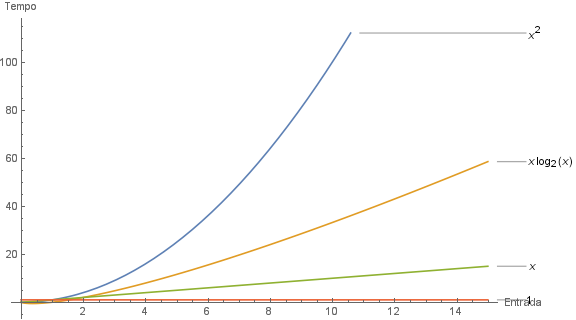
\includegraphics[width=.9\linewidth]{./img/ordens_grandeza.png}
\caption{\small Gráfico mostrando ordens de grandeza mais comuns de algoritmos}
\end{figure}

Pode-se verificar, colocando todos os algoritmos em análise, que os algoritmos
de complexidade quadrática ganham destaque no gráfico. Sendo esse um motivo que
até ofusca a visualização dos outros. Tal afirmação é observada no gráfico
abaixo, montado sobre a coleta de tempo de execução dos algoritmos em função
do tamanho da entrada.

\begin{figure}[htb]
\centering
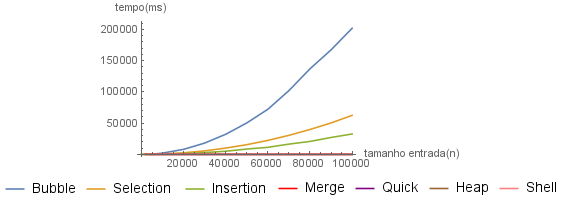
\includegraphics[width=.9\linewidth]{./img/all_random.png}
\caption{\small Performance de todos os  algoritmos em dados aleatórios}
\end{figure}

\chapter{Análise dos algoritmos quadráticos}
\label{sec-4-1}
Os algoritmos de complexidade quadrática se mostraram ineficientes como
consequência os mais lentos, como esperado dada a teoria existente. Abaixo
seguem-se as análises contemplando todos os algoritmos em suas diversas formas
de ordenação.

\begin{figure}[htb]
\centering
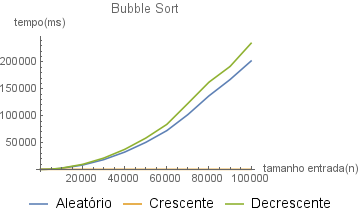
\includegraphics[width=.9\linewidth]{./img/bubble_all.png}
\caption{Performance do Bubble Sort}
\end{figure}

\begin{figure}[htb]
\centering
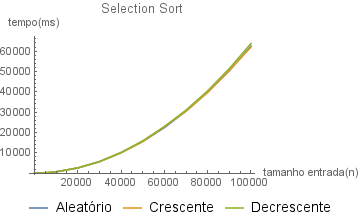
\includegraphics[width=.9\linewidth]{./img/selection_all.png}
\caption{Performance do Selection Sort}
\end{figure}

\begin{figure}[htb]
\centering
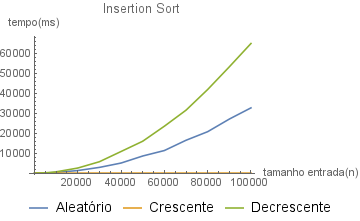
\includegraphics[width=.9\linewidth]{./img/insertion_all.png}
\caption{Performance do Insertion Sort}
\end{figure}

\begin{figure}[htb]
\centering
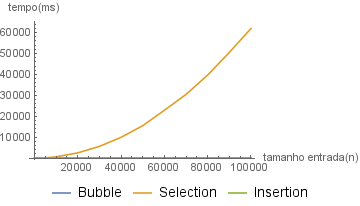
\includegraphics[width=.9\linewidth]{./img/quadratic_crescent.png}
\caption{\small Performance dos algoritmos quadráticos em dados crescentes}
\end{figure}

\begin{figure}[htb]
\centering
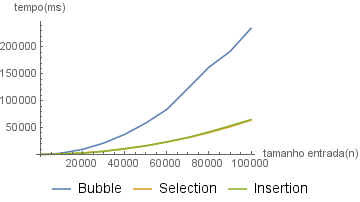
\includegraphics[width=.9\linewidth]{./img/quadratic_decrescent.png}
\caption{\small Performance dos algoritmos quadráticos em dados decrescentes}
\end{figure}

\begin{figure}[htb]
\centering
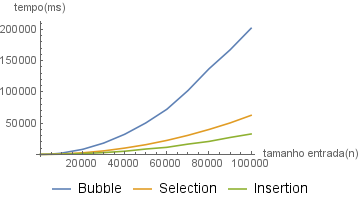
\includegraphics[width=.9\linewidth]{./img/quadratic_random.png}
\caption{\small Performance dos algoritmos quadráticos em dados aleatórios}
\end{figure}

\chapter{Análise dos algoritmos linear logaritmicos}
\label{sec-4-2}
Inicialmente, para mostrar com fidelidade o crescimento assintótico do gráfico
algumas mudanças foram feitas. Os algoritmos linear logaritmicos não mostram o
comportamento de crescimento esperado utilizando a função $ListLinePlot$.
Utilizando-se dessa função, ao plotar os dados do \emph{Merge Sort}, observou-se
que o gráfico demonstrava um crescimento linear ao olhar unicamente para os
pontos plotados.

\begin{figure}[htb]
\centering
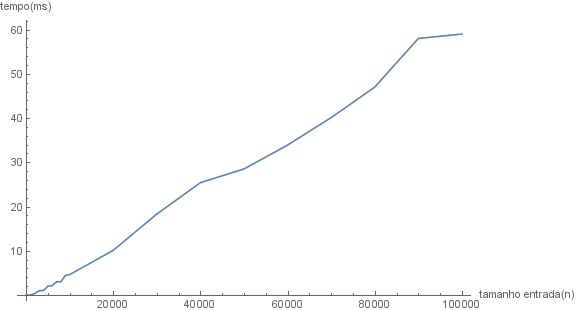
\includegraphics[width=.9\linewidth]{./img/old_merge_random.png}
\caption{Gráfico do \emph{Merge sort} utilizando \emph{ListLinePlot[\ldots{}]}}
\end{figure}

Ao utilizar a função \emph{ListLogPlot} pode-se obter um resultado fiel ao desejado,
ou seja, observa-se o crescimento logaritmico esperado do algoritmo testado.

\begin{figure}[htb]
\centering
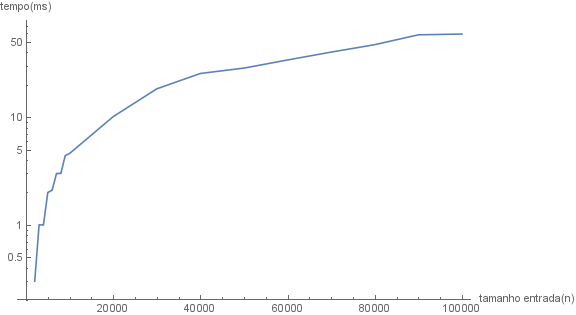
\includegraphics[width=.9\linewidth]{./img/merge_random.png}
\caption{Gráfico do \emph{Merge Sort} utilizando \emph{ListLogPlot[\ldots{}]}}
\end{figure}

Ademais, um algoritmo que, a princípio, parecia ter comportamento quadrático
foi, empiricamente, enquadrado em outra categoria: a linear logaritmica. O
\emph{Shell Sort} mostrou-se eficiente na ordenação com um \emph{gap} calculado como
$gap = 3 \cdot gap + 1$ e, ao gerar o gráfico, mostrou ser um algoritmo
pertencente a categoria desta seção. Portanto, conclui-se que, para esse
cálculo de intervalo o \emph{Shell Sort} se encaixa como algoritmo linear
logaritmico.

Por fim, conclui-se que os algoritmos linear logaritmicos de forma geral são
mais eficazes que os algoritmos de complexidade quadrática. Isso foi
demonstrado empiricamente, fato que pode ser observado nos gráficos
posteriores onde é visível que, dos algoritmos mais lentos utilizou-se menos
de 100 milisegundos para ordenar uma instância com cem mil elementos.

A comparação final dos quatro algoritmos quando pode ser vista na figura
4.17 para os dados aleatórios.

É visível a diferença de tempo de execução dos quatro algoritmos,
com exceção ao \emph{Shell} e ao \emph{Heap} que tem tempos parecidos para entradas
próximas a 20000. Com isso é possível classificar, quanto ao tempo utilizado
para ordenar, esses algoritmos. Do mais rápido para o mais lento obtém-se a
seguinte lista:

\begin{enumerate}
\item Quick
\item Merge
\item Shell
\item Heap
\end{enumerate}

Portanto, pode-se observar que o \emph{Heap} é o algoritmo mais lento entre os
linear logaritmicos, sendo menos eficiente que o \emph{Shell Sort} em todas as
situações testadas. Além disso, é notório que o \emph{Quick Sort} se manteve como
algoritmo mais eficiente dentre os demais utilizando um método de escolha de
pivô trivial.

Abaixo pode se observar o resultado dos testes empíricos sobre os algoritmos
linear logaritmicos em diferentes tipos de dados.

\begin{figure}[htb]
\centering
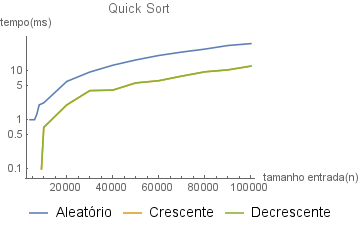
\includegraphics[width=.9\linewidth]{./img/quick_all.png}
\caption{Performance do Quick sort}
\end{figure}

\begin{figure}[htb]
\centering
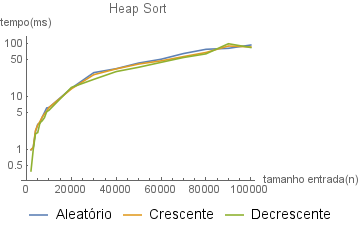
\includegraphics[width=.9\linewidth]{./img/heap_all.png}
\caption{Performance do Heap sort}
\end{figure}

\begin{figure}[htb]
\centering
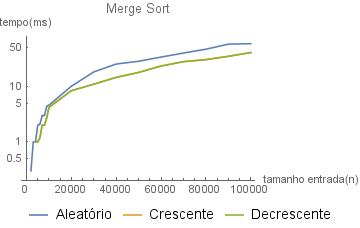
\includegraphics[width=.9\linewidth]{./img/merge_all.png}
\caption{Performance do Merge sort}
\end{figure}

\begin{figure}[htb]
\centering
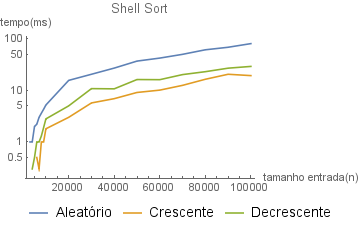
\includegraphics[width=.9\linewidth]{./img/shell_all.png}
\caption{Performance do Shell sort}
\end{figure}

\begin{figure}[htb]
\centering
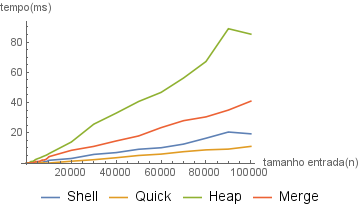
\includegraphics[width=.9\linewidth]{./img/logarithmic_crescent.png}
\caption{\small Performance dos linear logaritmicos em dados crescentes}
\end{figure}

\begin{figure}[htb]
\centering
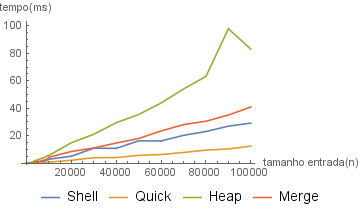
\includegraphics[width=.9\linewidth]{./img/logarithmic_decrescent.png}
\caption{\small Performance dos linear logaritmicos em dados decrescentes}
\end{figure}

\begin{figure}[htb]
\centering
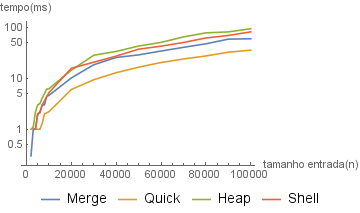
\includegraphics[width=.9\linewidth]{./img/logarithmic_random.png}
\caption{\small Performance dos linear logaritmicos em dados aleatórios}
\end{figure}

\part{Anexos}
\label{sec-5}
O trabalho acompanha uma pasta intitulada \emph{algorithms} onde contém todos os
algoritmos de ordenação e seus respectivos testes.

Se necessário, a implementação dos algoritmos de ordenação pode ser também
encontrada em: \url{https://github.com/rafaelcn/algorithms}.

\part{Referências}
\label{sec-6}
\noindent
CORMEN, Thomas et al. \textbf{Algoritmos}. 3. ed. Elsevier, 2012.

\noindent
TOSCANI, Laira, VELOSO, Paulo. \textbf{Complexidade de Algoritmos : análise,
projeto e métodos}. 3. ed. Bookman, 2012.

\noindent
SEDGEWICK, Robert. \textbf{A New Upper Bound for Shellsort}. Journal of Algorithms,
1986

\noindent
SKIENA, Steven. \textbf{Sorting and Searching}. Springer, 2008.

\noindent
Wolfram Development Platform. Acesso disponível em:
\textless{}\url{https://develop.wolframcloud.com/app/}\textgreater{}

\noindent
Rosetta Code. \textbf{Quick Sort}. Acesso disponível em:
\textless{}\url{https://rosettacode.org/wiki/Sorting_algorithms/Quicksort}\textgreater{}
% Emacs 25.3.1 (Org mode 8.2.10)
\end{document}
